\chapter{Background and Related Work}\label{relatedWork}

%CRN backgrounds, motivation
Traditional analog model for spectrum management resulted into the inefficient utilization of most radio frequency spectrum~\cite{valenta2010survey}. While several mobile network spectrum bands are highly congested, other spectrum bands like TV space and non-commercial radio bands are overly under-utilized. Moreover, these utilization varies depending on time and place resulting into spectrum hole~\cite{tandra2009spectrum}. Subsequently, the notion of cognitive radio was proposed to exploit these temporal and spatial spectrum holes.

%CR definition
\section{Cognitive Radio Definition}
Cognitive radio is a special kind of radio with two unique attributes, cognitive capability and reconfigurability~\cite{akyildiz2006next, thomas2005cognitive, haykin2005cognitive}. Cognitive capability enables cognitive radio to sense its radio environment. The radio environment sensing process involves observing the power in various spectrum bands as well as identifying temporal and spatial spectrum holes~\cite{akyildiz2006next}. On the other hand, reconfigurability helps cognitive radio to communicate over various spectrum bands to improve spectrum utilization based on its spectrum awareness~\cite{jondral2005software}.

Based on these two special characteristics, the primary objective of cognitive radio can be best understood from its widely adopted definition~\cite{federal2005notice}:

\begin{quote}
A cognitive radio is a radio or system that senses its operational electromagnetic environment and can dynamically and autonomously adjust its radio operating parameters to modify system operation, such as maximize throughput, mitigate interference, facilitate interoperability, access secondary markets.
\end{quote}

Given the fixed nature of traditional spectrum allocation, the primary challenge of cognitive radio is to exploit spectrum holes in the licensed band while not causing any interruption to the licensed users. Therefore, while using a temporally and/or spatially free spectrum, if the licensed user starts using the corresponding spectrum, the cognitive radio must have the capability to switch to another spectrum or change its other transmission parameters to avoid interruption with the licensed user. Next, we will see how does a cognitive radio achieve this in greater detail.

\subsection{How does a cognitive radio physically work}

\begin{figure}[!htbp]
\begin{center}
    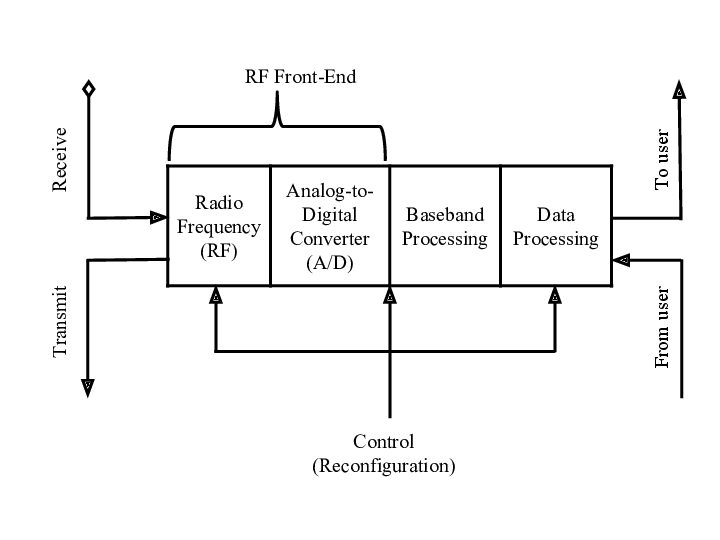
\includegraphics[scale=0.5]{myFigures/PhysicalCR}
    \caption{Cognitive radio transceiver (redrawn from~\cite{jondral2005software})}
    \label{fig:PhysicalCR}
\end{center}
\end{figure}

As shown in Figure~\ref{fig:PhysicalCR}~\cite{jondral2005software}, the cognitive radio transceiver is consisted of a radio front-end and a processing unit~\cite{akyildiz2006next}. The most important fact that distinguishes cognitive radios from other traditional radios is cognitive radio's ability to reconfigure itself via a control bus parameterizing both the radio front-end and processing units~\cite{jondral2005software}. The radio front-end amplifies and mixes the received signal and then converts it from analog to digital signal. The processing unit doing the job of baseband and data processing is quite similar to conventional radio transceivers. Nonetheless, the unique design of cognitive radio's front end also attributes to its novelty, and therefore, we will discuss the radio front-end up next.

\begin{figure}[!htbp]
\begin{center}
    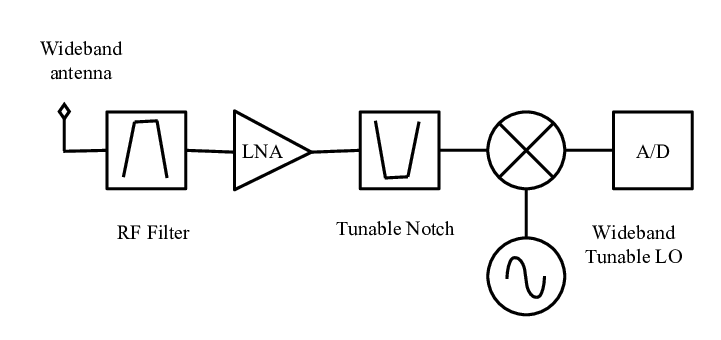
\includegraphics[scale=0.5]{myFigures/RFFrontEnd}
    \caption{Wideband RF/analog front-end architecture for cognitive radio (redrawn from~\cite{cabric2004implementation})}
    \label{fig:RFFrontEnd}
\end{center}
\end{figure}

The radio front-end of a cognitive radio is illustrated in Figure~\ref{fig:RFFrontEnd}~\cite{cabric2004implementation}. It has a wideband sensing capability mainly due to its components like wideband antenna, power amplifier, and adaptive filter. This wideband sensing capability of the radio front end enables cognitive radio to tune to any part of a wide spectrum band. This capability also helps cognitive radio to measure any spectrum information of radio surroundings. To accomplish all this, a wideband radio front-end needs to have following components~\cite{akyildiz2006next}:

\begin{itemize}
    \item \textbf{RF filter:} The RF filter chooses the appropriate (low, high, or bandpass) spectrum band by filtering out any other frequency components from the received RF signal.
    \item \textbf{Low noise amplifier (LNA):}
    \item \textbf{Mixer:}
    \item \textbf{Voltage-controlled oscillator (VCO):}
    \item \textbf{Phase locked loop (PLL):}
    \item \textbf{Channel selection filter:}
    \item \textbf{Automatic gain control (AGC):}
\end{itemize}
%CRN definition
%Research Categories in CRNs
    %Dynamic Spectrum Access issues in CRNs
        %Spectrum sensing
        %Spectrum management
        %Spectrum mobility
        %Spectrum sharing
    %Upper layer protocol design for CRNs
        %Routing protocols for CRNs
        %Transport layer protocols for CRNs
        %Cross layer approach
    %CRN security
    %CMRNs  

Existing studies on CMRNs mainly investigate how to incorporate multiple radios in dynamic spectrum sharing scenario. These studies mainly propose medium access control protocols~\cite{cormio2009survey, de2012survey}, routing protocols~\cite{zhu2008stod, feng2009joint}, and channel assignment~\cite{ahmadi2012distributed, zhong2014capacity} for CMRNs. Zhu et al., present a spectrum-tree based on-demand routing protocol that considers multi-radio nodes~\cite{zhu2008stod}. Such nodes belong to multiple spectrum-trees and are called overlapping nodes. As these nodes simultaneously work in different spectrum-trees, they can be used for inter-spectrum routing. The study shows that the proposed approach significantly reduces the average end-to-end delay.  Besides, Feng et al., propose a novel spectrum handoff scheduling approach for multi-hop CMRNs~\cite{feng2009joint}. This study presents a routing protocol with the help of aging-based priority assignment to minimize the latency. Thus none of these approaches addresses the problem of overcoming throughput degradation problem in CMRNs.

Ahmadi et al., present one of the earliest CRN studies involving multiple radios, which considers two sender radios for each secondary user~\cite{ahmadi2012distributed}. This study strives to solve channel assignment problem for the scenario. However, as there is only one receiver radio for each user in the proposed network model and channels are assigned to the receiver radio, the corresponding channel assignment problem becomes close to the single-radio channel assignment problem. This is because, as in single-radio scenario, only one channel needs to be assigned for each receiver node and the node can not exploit multiple available channels while receiving packets. Further, the study always uses a fixed number of transmitter radios (two) and do not investigate performance of the network for varying numbers of radios.

Another CMRN study~\cite{zhong2014capacity} by Zhong et al., aims to solve the channel assignment problem for CMRNs. Here, their proposed channel assignment approach assigns multiple channels among multiple radios available for secondary users. Despite ranking channels, while assigning them among radios, the approach does not consider the state of those radios. Besides, the paper does not provide any analysis on throughput with an increase in the number of radios.

The analysis of any performance metric based on an increase in the number of radios in CRNs is first presented in the study~\cite{li2014deterministic} by Li et al., to the best of our knowledge. The study presents a rendezvous channel establishment approach for CMRNs. It shows that the maximum time to rendezvous reduces with an increase in the number of radios used in CRNs. However, the study does not provide any solution on how these radios will be used for data transmission and its subsequent effect on performance metrics such as throughput and delay.

Later, Khan et al.,~\cite{khan2015towards} propose another CMRN architecture where each secondary user employs multiple radios for data transmission. The study shows that per packet average end-to-end delay gets improved at the cost of throughput degradation with an increase in the number of radios. This study does the radio-channel assignment in a random manner and does not avoid inter-user channel interface. Thus, this study fails to improve throughput with an increase in the number of radios.

In summary, none of the existing studies focuses on enhancing throughput in CMRNs. Therefore, we attempt to propose a new channel assignment approach to enhance throughput in CMRNs in this paper. Before presenting the approach, we first elaborate our system model and problem formulation.
\endinput
